\section{Modelado de datos}

Para la persistencia de la información se ha optado por MongoDB, una base de datos NoSQL orientada a documentos que aporta gran flexibilidad para evolucionar el esquema ágilmente. Aunque no es estrictamente necesario al usar MongoDB, se ha optado por utilizar la librería Mongoose como ODM para definir esquemas, tipos de datos y reglas de validación para facilitar el manejo de los datos y garantizar la integridad de estos.

Así, se han estructurado los datos en diferentes colecciones, cada una de las cuales guarda registros con varios campos de diferentes tipos de datos. El modelado de datos sigue el siguiente esquema.

\begin{figure}[H]
\centering
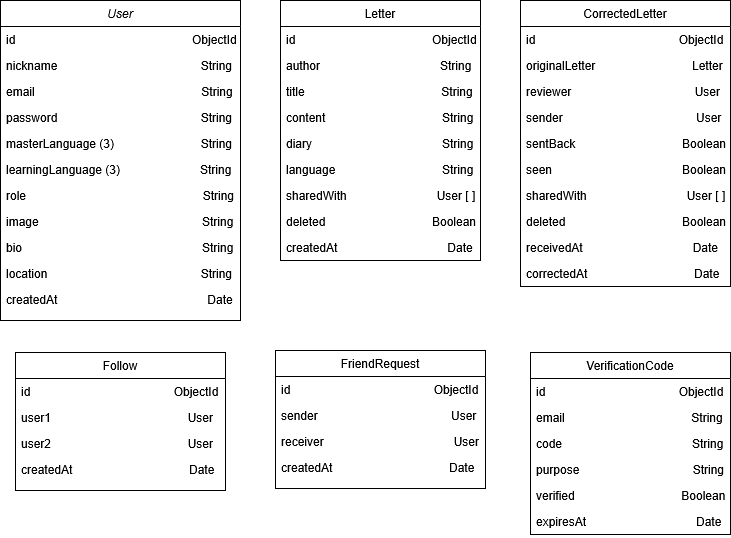
\includegraphics[width=0.8\textwidth]{./imagenes/letterexDB.png}
\caption{Estructura de Datos}
\label{fig:letterexDB}
\end{figure}

En el diseño destaca el uso del ObjectId, un identificador hexadecimal de 12 bytes que garantiza unicidad y permite la indexación eficiente basada en \textit{timestamps}. Además, facilita la vinculación mediante referencias entre colecciones. Cabe mencionar que, aunque internamente se usa \texttt{\_id}, el backend lo transforma en \texttt{id} antes de enviarlo al frontend para ofrecer una interfaz más limpia y desacoplada.

A continuación, se describen las colecciones del sistema:

\begin{itemize}
\item \textbf{Usuario (User):} gestiona la identidad y el perfil del usuario. Incluye su nombre de usuario, email, rol, imagen de perfil, biografía, localidad, contraseña, los idiomas que aprende y conoce (limitados a tres entradas por optimización técnica) y la fecha de creación.
Por seguridad, no se almacena el texto plano de la contraseña, sino que se utiliza la librería \textbf{bcrypt} con un factor de coste (\textit{salting}) de 10 para cifrar la clave antes de su persistencia. El salting es un parámetro que determina la complejidad computacional del hash para dificultar ataques de fuerza bruta al aumentar el tiempo de procesamiento necesario. Se ha escogido 10 por ser el estándar actual en la industria, aquel que se considera el punto de equilibrio óptimo entre seguridad y rendimiento. Cada vez que se quiera comprobar la contraseña, se hashea la entrada con el mismo salting y se compara el resultado con el valor guardado en la base de datos, de forma que ni el administrador ni un atacante pueda tener acceso a la contraseña.

\item \textbf{Carta (Letter):} almacena los textos originales. Contiene el author (referencia al usuario creador), título, contenido, diario, idioma y fecha de creación. También incluye un array de referencias a los usuarios con que se comparte la carta (\textit{sharedWith}) y un campo \textit{deleted} para el borrado lógico, permitiendo que los receptores conserven sus correcciones.

\item \textbf{Carta Corregida (CorrectedLetter):} gestiona el flujo de revisión. Vincula la corrección a la carta original mediante le referencia \textit{originalLetter}, además de referenciar al revisor o receptor de la carta (\textit{reviewer}) y a su autor (\textit{sender}). Controla los estados de envío de vuelta mediante el booleano \textit{sentBack}, y de si el receptor vio ya la nueva carta que le llegó con el booleano \textit{seen}, de forma que en el frontend se puedan crear etiquetas de "Nuevo" a modo de notificación. También, guarda la fecha de envío y de corrección (envío de vuelta) de la carta.

\item \textbf{Amistad (Follow):} gestiona el grafo social mediante referencias a \textit{user1} (seguidor) y \textit{user2} (seguido), facilitando el intercambio de correcciones y el listado de amigos y usuarios sugeridos.

\item \textbf{Solicitud de Amistad (FriendRequest):} capa intermedia para peticiones de amistad entre un usuario \textit{sender} y un usuario \textit{receiver}. Es una colección efímera: al aceptar o rechazar, el documento se elimina, creando el vínculo en la colección \textit{Follow} en caso de aceptación.

\item \textbf{Código de Verificación (VerificationCode):} entidad de apoyo para la validación de registros y recuperación de claves. Almacena el código hasheado, el email del usuario implicado, un campo \textit{verified} que indica si ya ha sido utilizado, y un campo \textit{purpose} que indica si sirve para un registro o para una recuperación de contraseña. Además, se utiliza un índice TTL (Time To Live) en el campo \textit{expiresAt}, que sirve para que MongoDB elimine automáticamente los códigos al cabo de 7 minutos de su creación.

\end{itemize}